\chapter{Mezclar y disolver}\label{ch:g2:mixing-and-dissolving}

Un terrón de azúcar cae en una taza de té caliente. Una cucharilla
remueve, el terrón se deshace y, al cabo de un momento, ya no se ve
nada: el té tiene exactamente el mismo aspecto que antes. Y, sin
embargo, ahora sabe dulce. El azúcar no se ha ido: está escondido en el
té. Este capítulo trata de juntar cosas, y de las cosas que parecen
desaparecer cuando lo hacemos.

\begin{omfigure}
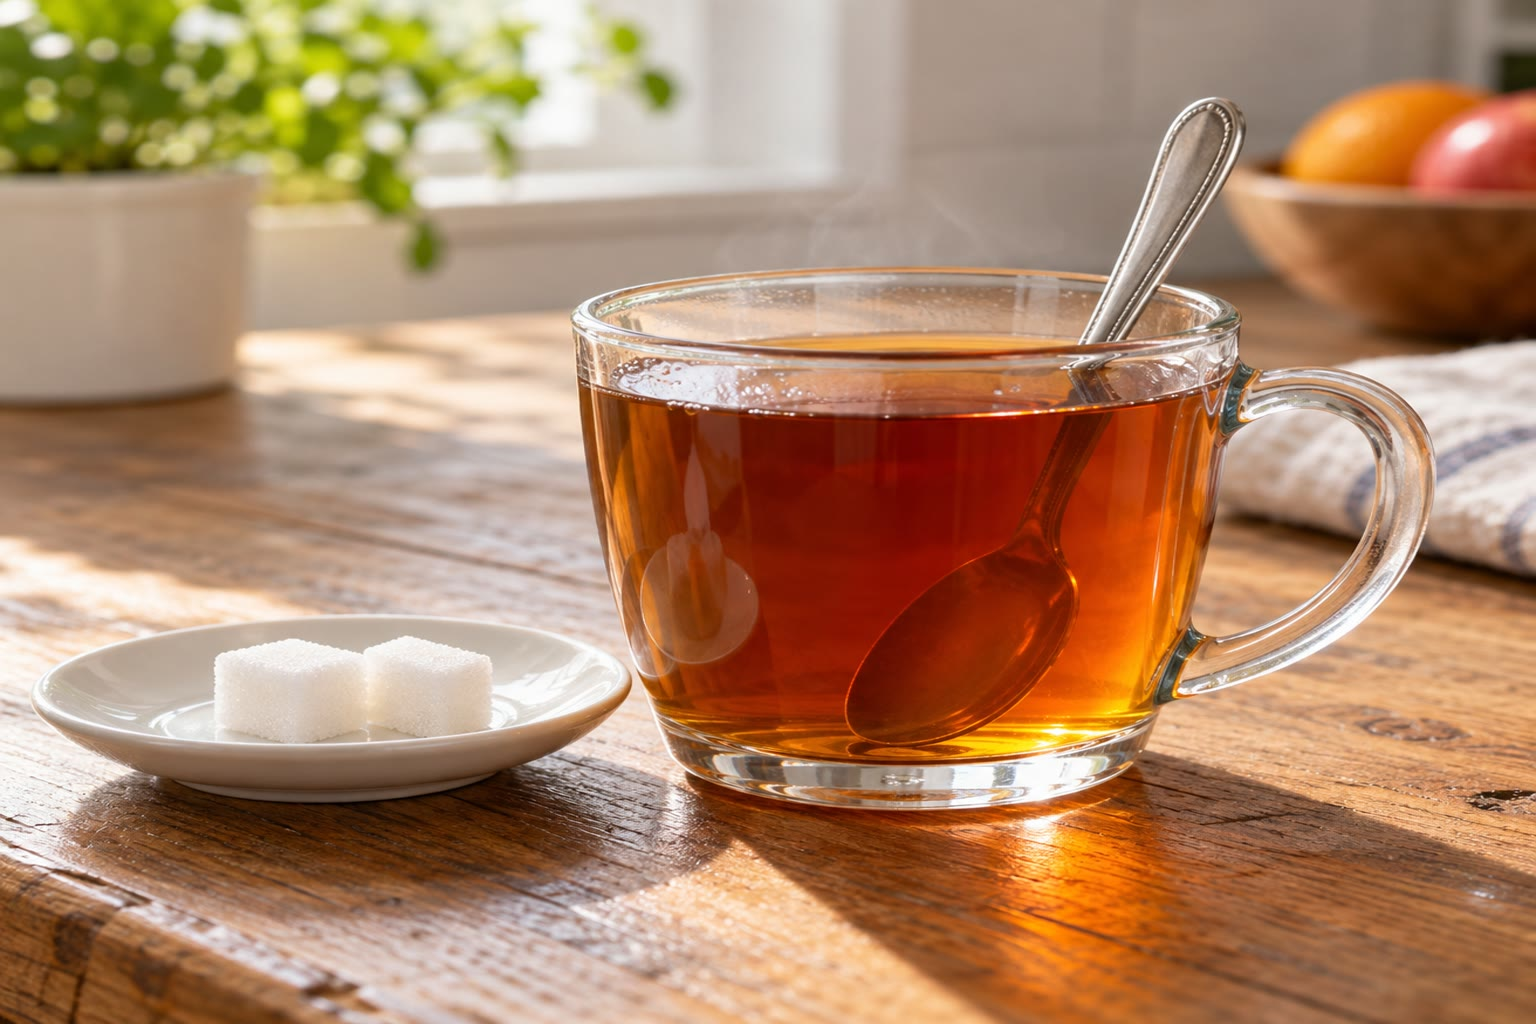
\includegraphics[width=0.55\linewidth]{images/book1/ai/g2-tea-sugar.jpg}

{\small Una taza de té y dos terrones de azúcar. Al removerlo, el azúcar
desaparece de la vista, pero no del sabor.}
\end{omfigure}

\section{Mezclar cosas}

\begin{definition}[Mezclar]\label{def:g2:mixing-and-dissolving:mix}
Decimos que \emph{mezclamos}\index{mezclar} cuando juntamos cosas
distintas y, a menudo, las removemos. Lo que obtenemos es una mezcla de
esas cosas.
\end{definition}

\begin{example}[Un cuenco de muesli]\label{ex:g2:mixing-and-dissolving:muesli}
En un mismo cuenco se echan copos de avena, pasas, frutos secos y
semillas: eso es una mezcla. Si miramos de cerca, todavía se ve cada
ingrediente, y podemos volver a sacarlo con los dedos: una pasa sigue
siendo una pasa, y una nuez sigue siendo una nuez.
\end{example}

\begin{example}[Jarabe en agua]\label{ex:g2:mixing-and-dissolving:syrup}
También se pueden \omterm{def:g2:mixing-and-dissolving:mix}{mezclar} dos líquidos. Un jarabe rojo vertido en un
vaso de agua baja formando remolinos de color; después de remover, todo
el vaso queda de un rosa uniforme. A simple vista ya no se distinguen
el jarabe y el agua.
\end{example}

\begin{omfigure}
\begin{minipage}[t]{0.48\linewidth}\centering
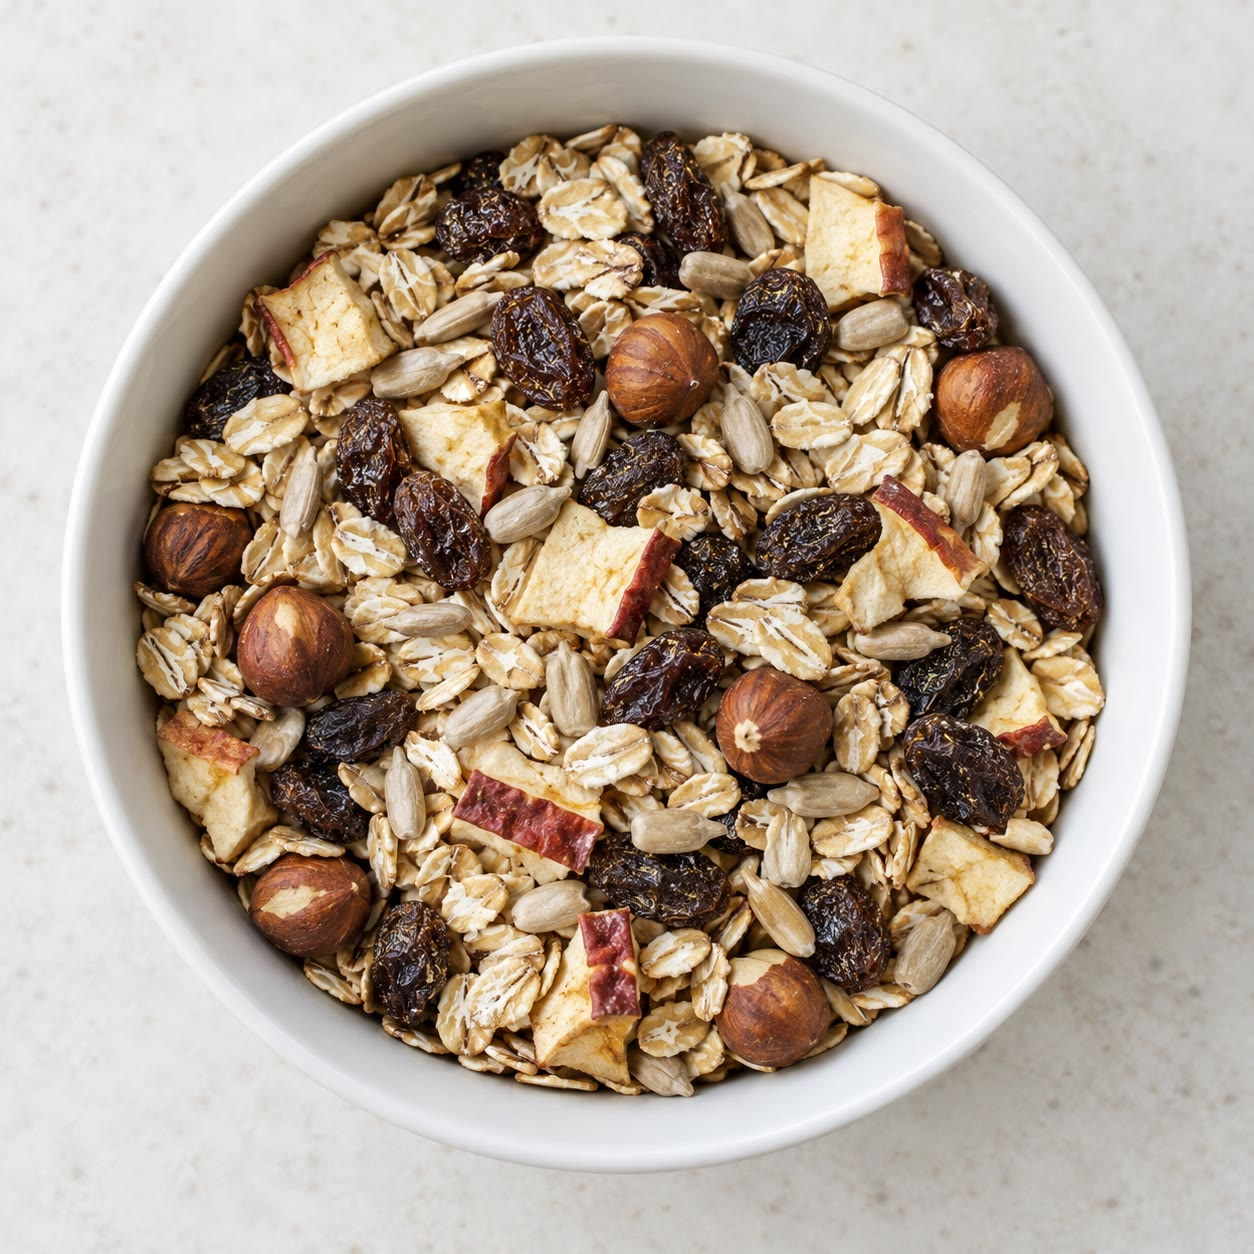
\includegraphics[width=\linewidth,height=4.6cm,keepaspectratio]{images/book1/ai/g2-muesli.jpg}

{\small El muesli: una mezcla en la que todavía se ve cada parte.}
\end{minipage}\hfill
\begin{minipage}[t]{0.48\linewidth}\centering
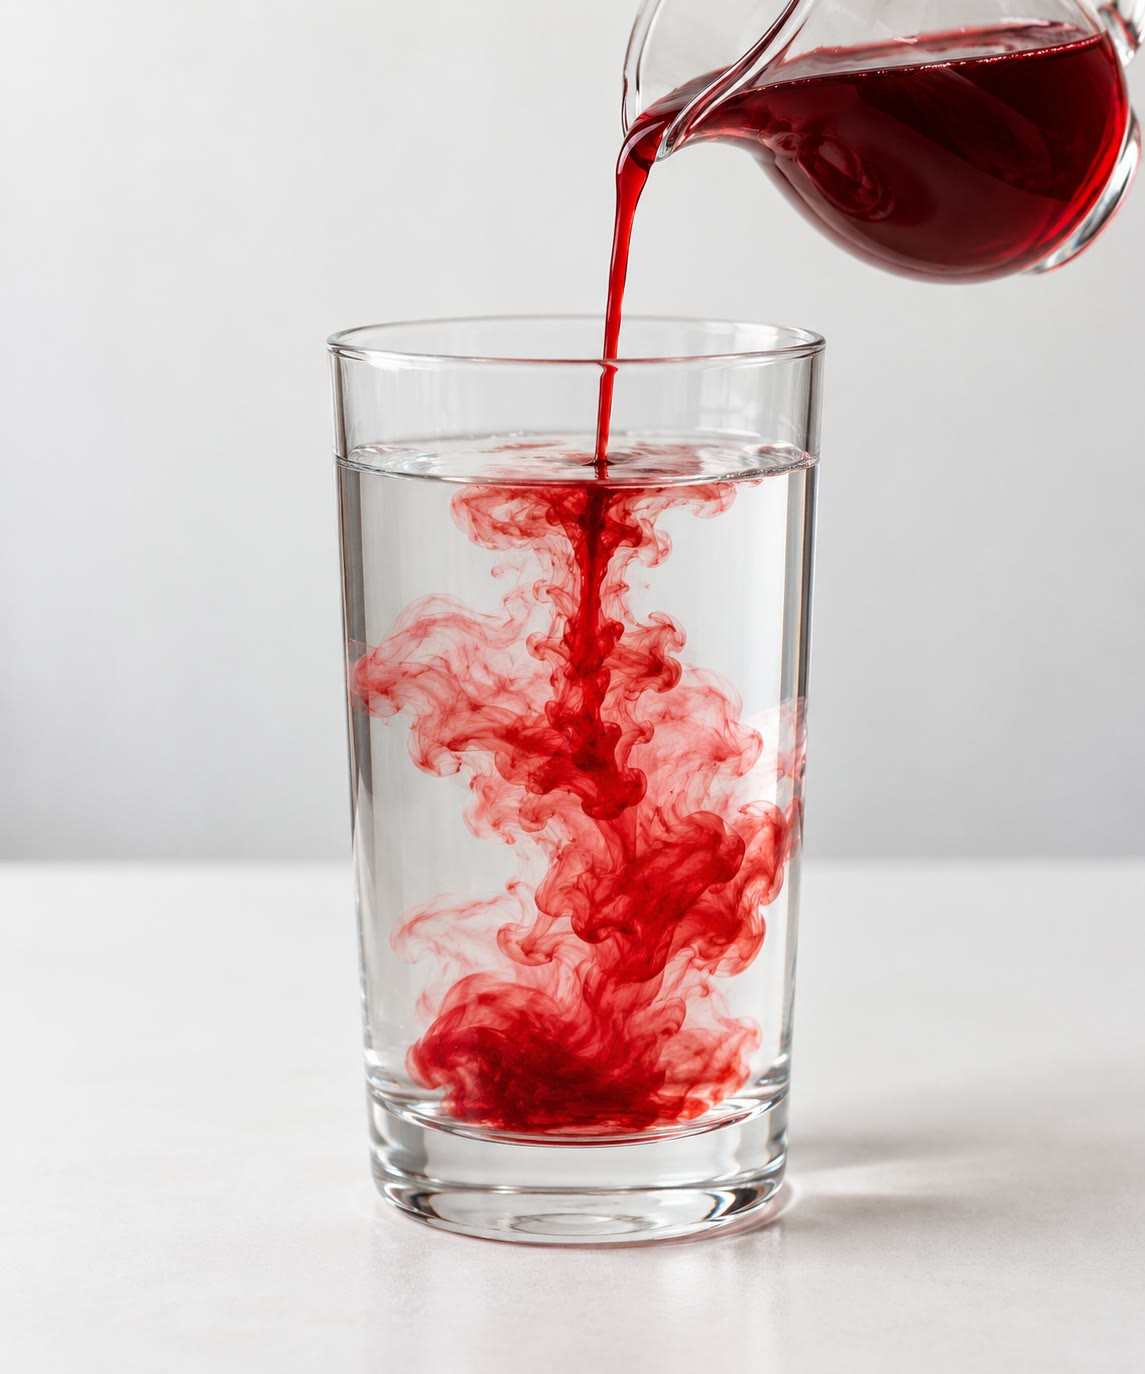
\includegraphics[width=\linewidth,height=4.6cm,keepaspectratio]{images/book1/ai/g2-syrup-in-water.jpg}

{\small Jarabe vertido en agua: dos líquidos que se \omterm{def:g2:mixing-and-dissolving:mix}{mezclan}.}
\end{minipage}
\end{omfigure}

\begin{remark}[Al mezclar no se destruye nada]\label{rem:g2:mixing-and-dissolving:nothing-lost}
Cuando se \omterm{def:g2:mixing-and-dissolving:mix}{mezclan} cosas, no se pierde nada y no se fabrica nada nuevo.
La avena, las pasas y los frutos secos siguen todos en el cuenco. Un
capítulo posterior enseña a separar de nuevo una mezcla.
\end{remark}

\section{Cosas que se disuelven}

\begin{definition}[Disolverse; disolución]\label{def:g2:mixing-and-dissolving:dissolve}
Un sólido se \emph{disuelve}\index{disolverse} en agua cuando, \omterm{def:g2:mixing-and-dissolving:mix}{mezclado}
con el agua y removido, desaparece de la vista y deja el líquido
\emph{transparente}, es decir, que se puede ver a través de él. El
azúcar y la sal se disuelven en agua. El líquido transparente que
obtenemos se llama
\emph{disolución}\index{disolucion@disolución}: el agua con azúcar es una
disolución de azúcar, y el agua salada, una disolución de sal.
\end{definition}

\begin{example}[Un terrón de azúcar en un vaso de agua]\label{ex:g2:mixing-and-dissolving:cube}
Dejamos un terrón de azúcar en el fondo de un vaso de agua quieta. Sus
esquinas se ablandan, se va haciendo más pequeño y de él suben por el
agua unas estelas onduladas. Si removemos, desaparece en menos de un
minuto. Si no removemos, desaparece igualmente, pero mucho más despacio.
\end{example}

\begin{remark}[Transparente no es lo mismo que incoloro]\label{rem:g2:mixing-and-dissolving:clear}
El té es marrón y el agua con jarabe es rosa, pero podemos ver a través
de los dos: son transparentes. Una \omterm{def:g2:mixing-and-dissolving:dissolve}{disolución} puede tener color. Lo que
una \omterm{def:g2:mixing-and-dissolving:dissolve}{disolución} no tiene nunca son trocitos flotando ni una capa en el
fondo.
\end{remark}

\begin{method}[¿Se disuelve?]\label{met:g2:mixing-and-dissolving:test}
Para saber si un sólido se \omterm{def:g2:mixing-and-dissolving:dissolve}{disuelve} en agua:
\begin{enumerate}
  \item echa un poco del sólido en un vaso de agua;
  \item remueve y espera unos minutos;
  \item mira a través del vaso:
    \begin{itemize}
      \item transparente y sin nada en el fondo: el sólido se ha disuelto;
      \item turbio, o con una capa en el fondo: el sólido no se ha disuelto.
    \end{itemize}
\end{enumerate}
\end{method}

\section{Cosas que no se disuelven}

\begin{proposition}[La arena y la tiza no se disuelven]\label{prop:g2:mixing-and-dissolving:not}
Muchos sólidos no se \omterm{def:g2:mixing-and-dissolving:dissolve}{disuelven} en agua: la arena, la tiza, la tierra,
los guijarros, la harina. Si los removemos en agua, la enturbian; si
los dejamos reposar, bajan y se depositan en el fondo, y el agua de
encima vuelve a aclararse. Por mucho que removamos, nunca desaparecen.
\end{proposition}

\begin{example}[Un tarro de agua turbia]\label{ex:g2:mixing-and-dissolving:mud}
Si agitamos tierra del jardín en un tarro con agua, el agua se vuelve
marrón y turbia. Al cabo de una hora, la tierra y las piedrecitas forman
una capa oscura en el fondo, unas cuantas hojas secas flotan arriba y
el agua de en medio solo está un poco turbia. La tierra no se ha
disuelto.
\end{example}

\begin{omfigure}
\begin{minipage}[t]{0.48\linewidth}\centering
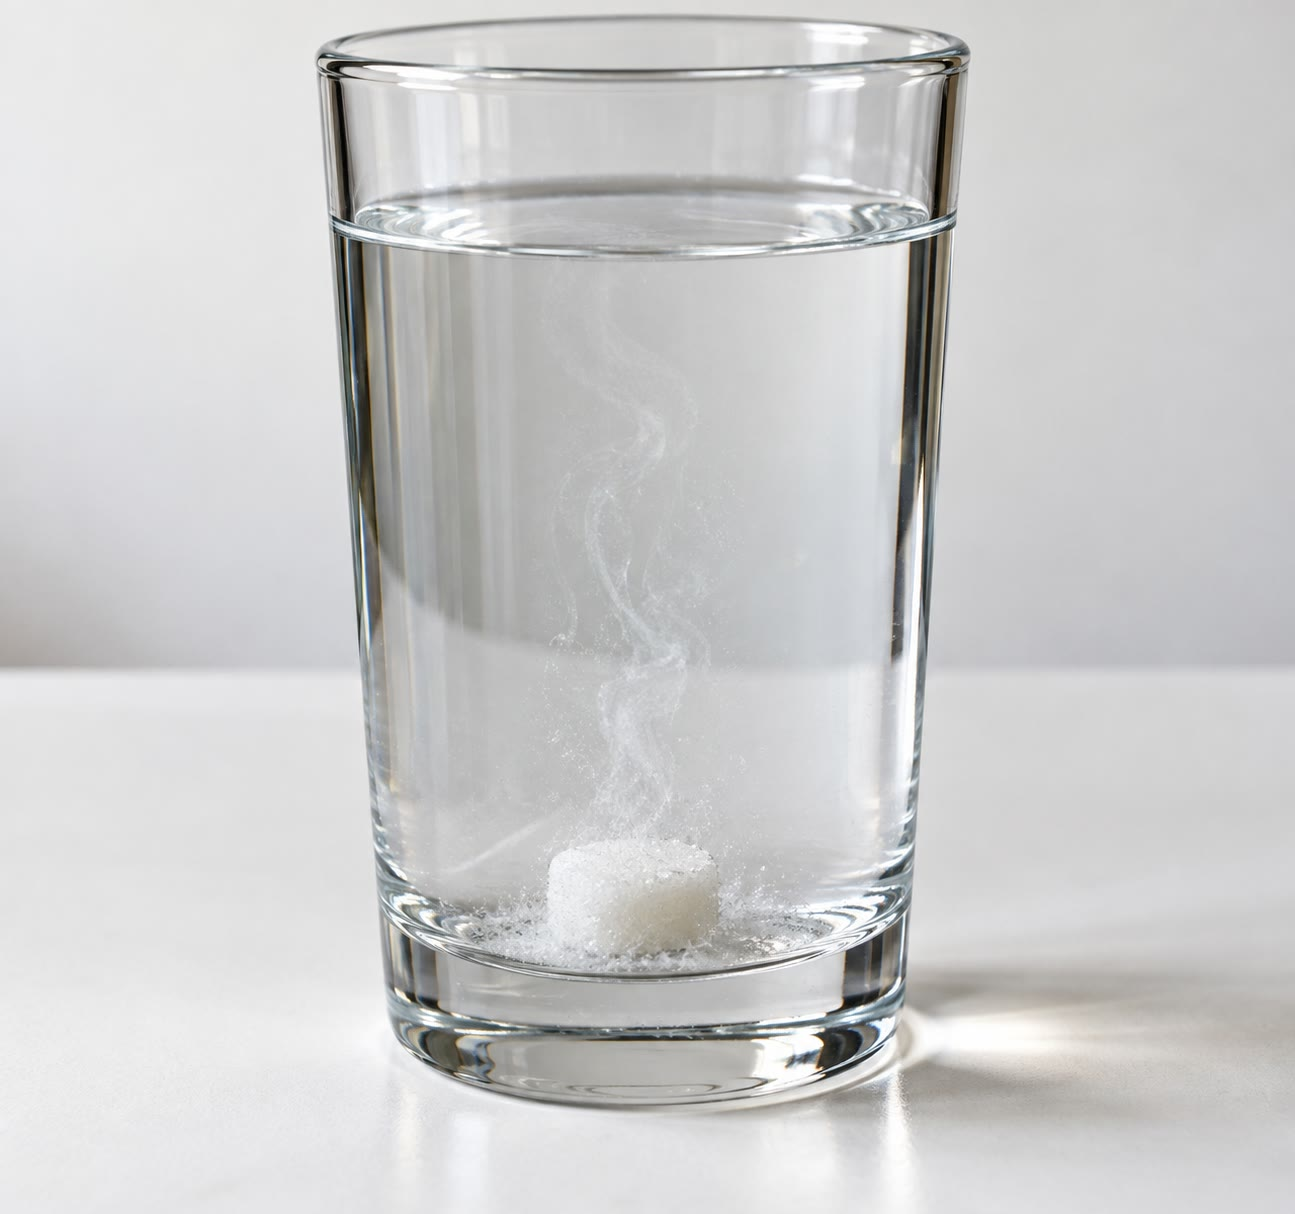
\includegraphics[width=\linewidth,height=4.6cm,keepaspectratio]{images/book1/ai/g2-sugar-cube-dissolving.jpg}

{\small El azúcar se \omterm{def:g2:mixing-and-dissolving:dissolve}{disuelve}: del terrón suben estelas.}
\end{minipage}\hfill
\begin{minipage}[t]{0.48\linewidth}\centering
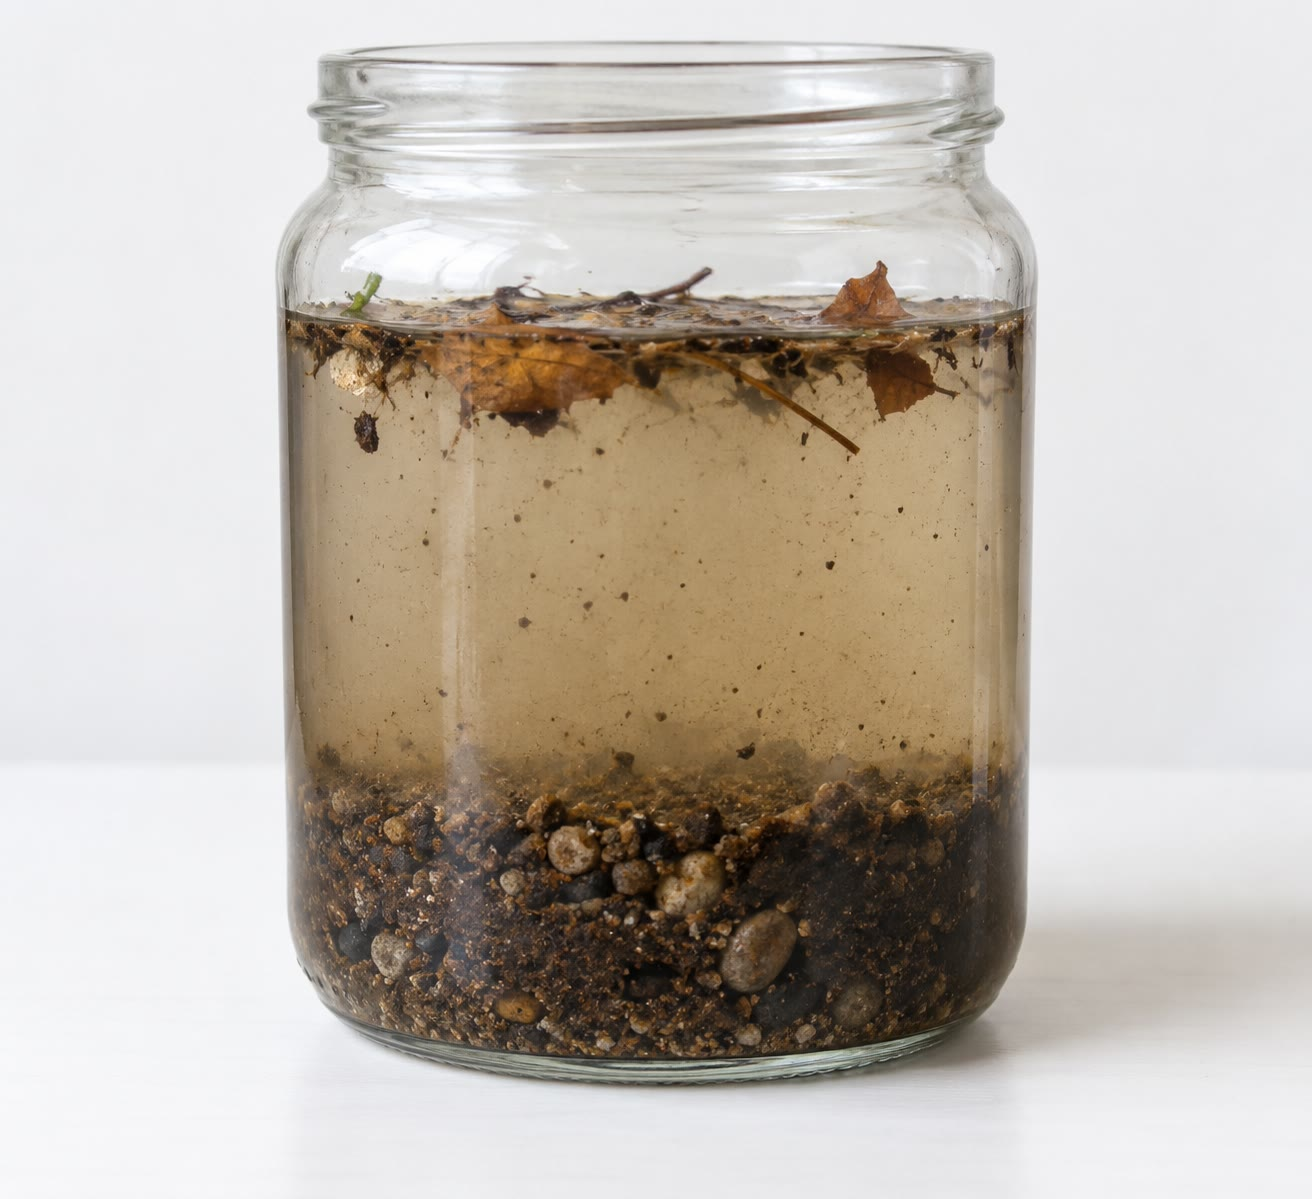
\includegraphics[width=\linewidth,height=4.6cm,keepaspectratio]{images/book1/ai/g2-muddy-jar.jpg}

{\small La tierra no se \omterm{def:g2:mixing-and-dissolving:dissolve}{disuelve}: se deposita en el fondo.}
\end{minipage}
\end{omfigure}

\begin{omfigure}
\begin{tikzpicture}[font=\small, scale=1.35]
  \pic[transform shape] at (0,0) {beaker={0.7}{omWater!70}};
  \fill[brown!55] (4.2,0) rectangle (5.8,0.22);
  \pic[transform shape] at (5,0) {beaker={0.7}{brown!12}};
  \fill[brown!55] (4.2,0) rectangle (5.8,0.22);
  \draw[omGlass, line width=0.7pt] (4.2,0.22) -- (4.2,0) -- (5.8,0) -- (5.8,0.22);
  \foreach \x/\y in {4.4/0.32,4.75/0.45,5.1/0.3,5.5/0.5,4.6/0.7,5.3/0.8,4.9/1.0}
    \fill[brown!60] (\x,\y) circle (0.025);
  \node[align=center, anchor=north] at (0,-0.15)
    {\textbf{azúcar} en agua, removido:\\ transparente, nada en el fondo};
  \node[align=center, anchor=north] at (5,-0.15)
    {\textbf{arena} en agua, removida:\\ turbia, una capa en el fondo};
  \draw[<-, omProp, thick] (6.0,0.11) -- (7.0,0.11)
    node[right, text=black] {la arena};
\end{tikzpicture}

{\small La prueba del \cref{met:g2:mixing-and-dissolving:test}: el
azúcar se \omterm{def:g2:mixing-and-dissolving:dissolve}{disuelve}; la arena, no.}
\end{omfigure}

\section{Lo que se disuelve sigue ahí}

\begin{proposition}[Un sólido disuelto sigue en el agua]\label{prop:g2:mixing-and-dissolving:still-there}
Cuando un sólido se \omterm{def:g2:mixing-and-dissolving:dissolve}{disuelve}, no se esfuma: queda repartido por toda el
agua, en trocitos demasiado pequeños para verlos. Dos pistas muestran
que sigue ahí:
\begin{itemize}
  \item el té con azúcar sabe dulce, y el agua del mar sabe salada;
  \item cuando el agua se seca, el sólido se queda.
\end{itemize}
\end{proposition}

\begin{remark}[En el laboratorio no se prueba nada]\label{rem:g2:mixing-and-dissolving:no-tasting}
Sabemos que el té es dulce porque el té es un alimento. En un
laboratorio nadie prueba nunca nada, ni siquiera un líquido que parezca
agua: la segunda pista, dejar que el agua se seque, es la que usan los
químicos.
\end{remark}

\begin{example}[Sal del mar]\label{ex:g2:mixing-and-dissolving:salt-pans}
En algunas costas soleadas se deja entrar el agua del mar en estanques
anchos y poco profundos. Día tras día, el sol seca el agua. Lo que queda
en el fondo es sal blanca, que se recoge con rastrillos en montones: la
sal que estaba disuelta en el mar. La sal de la mesa viene a menudo de
estas salinas.
\end{example}

\begin{omfigure}
\begin{tikzpicture}[font=\small, scale=1.25]
  % day 1: a saucer of salty water
  \fill[omWater!80] (0,0.18) ellipse (1.25 and 0.22);
  \draw[omGlass, line width=0.7pt] (-1.5,0.3) .. controls (-1.2,-0.15) and (1.2,-0.15) .. (1.5,0.3);
  \draw[omGlass, line width=0.5pt] (0,0.3) ellipse (1.5 and 0.28);
  \node[align=center, anchor=north] at (0,-0.35) {un platito de\\ agua salada};
  % the sun
  \fill[ocYellow] (3.4,1.45) circle (0.28);
  \foreach \a in {0,45,...,315}
    \draw[ocYellow!90!orange, thick] ($(3.4,1.45)+(\a:0.36)$) -- ($(3.4,1.45)+(\a:0.52)$);
  \draw[->, thick, omProp] (2.0,0.3) -- (4.8,0.3)
    node[midway, below, text=black, align=center] {unos días de sol\\ después};
  % later: a white crust
  \begin{scope}[xshift=6.3cm]
    \draw[omGlass, line width=0.7pt] (-1.5,0.3) .. controls (-1.2,-0.15) and (1.2,-0.15) .. (1.5,0.3);
    \draw[omGlass, line width=0.5pt] (0,0.3) ellipse (1.5 and 0.28);
    \foreach \x/\y in {-0.9/0.12,-0.6/0.2,-0.3/0.08,0/0.18,0.3/0.1,0.6/0.2,0.9/0.12,
                       -0.45/0.28,0.15/0.27,0.75/0.3,-0.75/0.31}
      \fill[white, draw=black!45, line width=0.2pt] (\x,\y) rectangle ++(0.11,0.07);
    \node[align=center, anchor=north] at (0,-0.35) {ya no queda agua:\\ sal blanca};
  \end{scope}
\end{tikzpicture}

{\small El agua se seca; la sal que estaba disuelta en ella se queda.}
\end{omfigure}

\begin{omfigure}
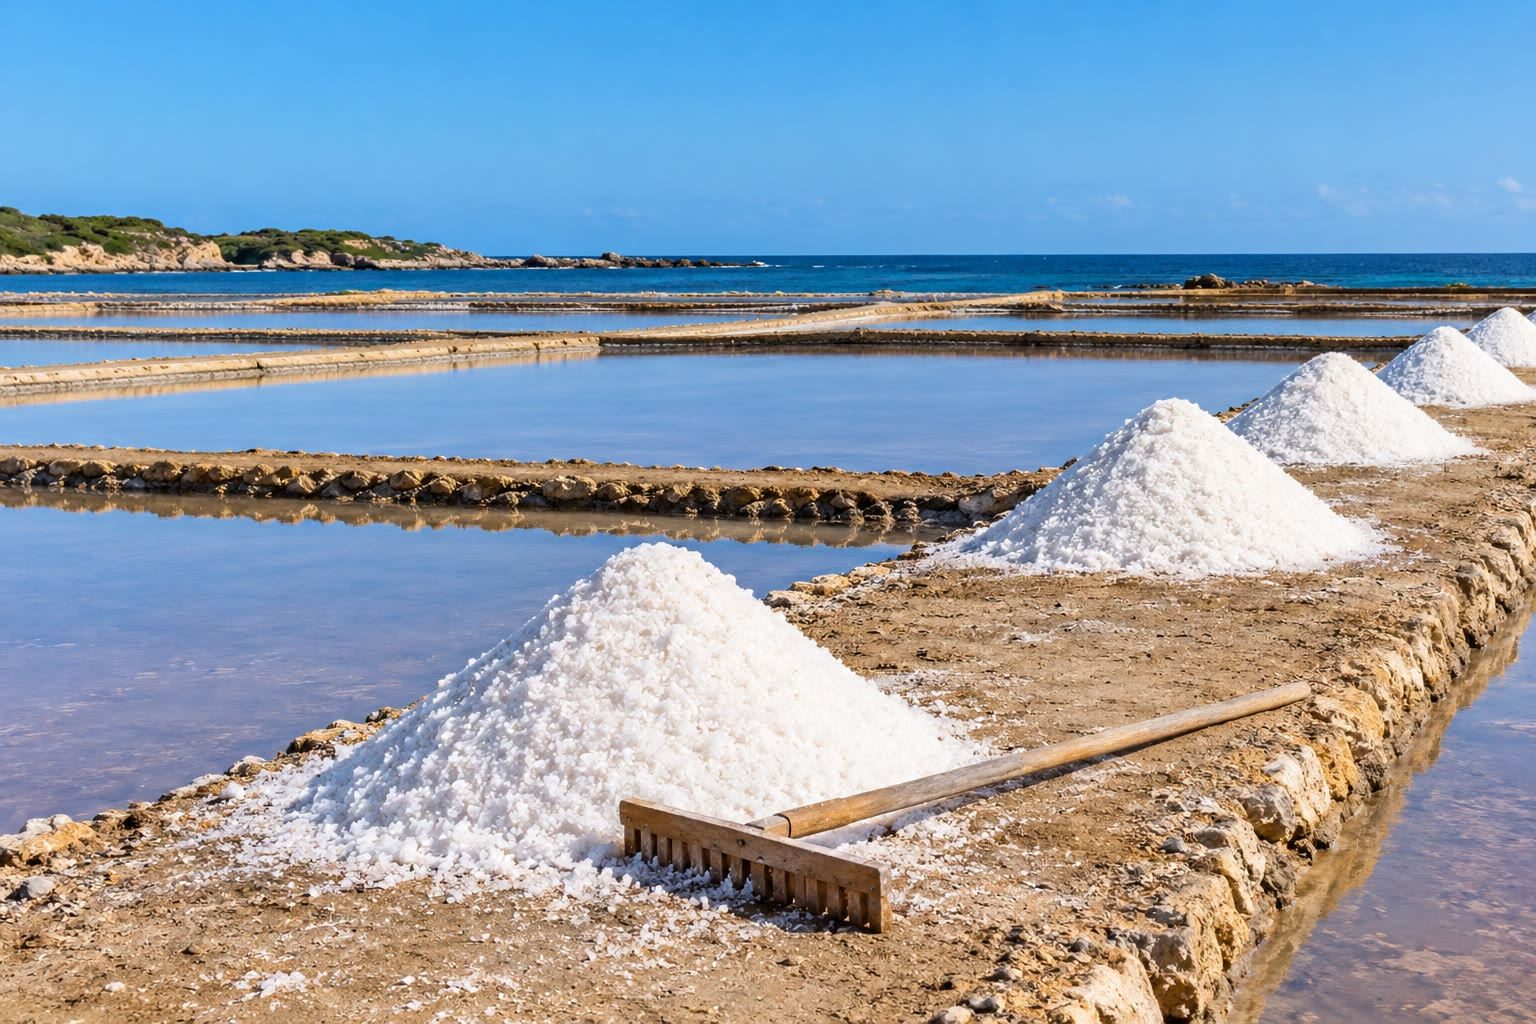
\includegraphics[width=0.62\linewidth]{images/book1/ai/g2-salt-pans.jpg}

{\small Salinas junto al mar: el sol seca el agua y la sal se queda en
montones blancos.}
\end{omfigure}

\begin{remark}[Disolverse no es fundirse]\label{rem:g2:mixing-and-dissolving:not-melting}
Mucha gente dice que el azúcar ``se derrite'' en el té. No es así:
derretirse, o fundirse, es lo que hace un cubito de hielo al sol, que
se convierte en líquido él solo, sin necesidad de agua. El azúcar en el
té necesita el agua, y el azúcar sigue en ella, repartido. La palabra
correcta es \emph{se \omterm{def:g2:mixing-and-dissolving:dissolve}{disuelve}}.
\end{remark}

\section{Ejercicios}

\begin{exercise}[$\star$]\label{exo:g2:mixing-and-dissolving:1}
¿Cuáles de estos sólidos se \omterm{def:g2:mixing-and-dissolving:dissolve}{disuelven} en agua y cuáles no? Azúcar,
arena, sal, tiza, guijarros.
\end{exercise}

\begin{exercise}[$\star$]\label{exo:g2:mixing-and-dissolving:2}
¿Qué es una \omterm{def:g2:mixing-and-dissolving:dissolve}{disolución}? Da dos ejemplos de este capítulo.
\end{exercise}

\begin{exercise}[$\star$]\label{exo:g2:mixing-and-dissolving:3}
¿Un cuenco de muesli es una mezcla? ¿Todavía puedes ver cada una de sus
partes?
\end{exercise}

\begin{exercise}[$\star$]\label{exo:g2:mixing-and-dissolving:4}
Removemos un polvo blanco en un vaso de agua. Al cabo de unos minutos,
el agua está turbia y se ha formado una capa blanca en el fondo. ¿Se ha
disuelto el polvo? Explícalo con el
\cref{met:g2:mixing-and-dissolving:test}.
\end{exercise}

\begin{exercise}[$\star$]\label{exo:g2:mixing-and-dissolving:5}
Un vaso de agua con jarabe es rosa. ¿Es transparente? ¿Es incoloro? ¿Es
una \omterm{def:g2:mixing-and-dissolving:dissolve}{disolución}?
\end{exercise}

\begin{exercise}[$\star$]\label{exo:g2:mixing-and-dissolving:6}
Después de remover, en una taza de té no se ve el azúcar. Da la pista
que muestra que el azúcar sigue ahí.
\end{exercise}

\begin{exercise}[$\star$]\label{exo:g2:mixing-and-dissolving:7}
En las salinas, ¿qué se lleva el sol y qué se queda?
\end{exercise}

\begin{exercise}[$\star$]\label{exo:g2:mixing-and-dissolving:8}
Tom dice: ``El azúcar se ha derretido en mi té''. ¿Qué palabra debería
usar en su lugar, y por qué?
\end{exercise}

\begin{exercise}[$\star\star$]\label{exo:g2:mixing-and-dissolving:9}
Mira la figura de los dos vasos de precipitados. Sin leer las palabras
de debajo, ¿cómo sabes qué vaso contiene la arena?
\end{exercise}

\begin{exercise}[$\star\star$]\label{exo:g2:mixing-and-dissolving:10}
Una gota de agua del grifo se seca sobre un plato negro y deja un
pequeño cerco blanco. ¿Qué nos dice esto sobre el agua del grifo?
\end{exercise}

\begin{exercise}[$\star\star$]\label{exo:g2:mixing-and-dissolving:11}
En el laboratorio, una profesora tiene dos vasos con un líquido
transparente e incoloro: uno contiene agua pura y el otro, agua salada.
Nadie puede probarlos. ¿Cómo puede averiguar cuál es cuál?
\end{exercise}
